% !TeX root = booklet-01.tex
\section{تقسیم طراحی و سطوح \lr{Abstraction}}
\label{sec:book-partitioning}
\subsection{چرا طراحی بزرگ را تقسیم می‌کنیم؟}
خواندن یک \lr{Inverter} با دنبال کردن دو ترانزیستور ممکن بود؛
در یک پردازنده، بررسی هم‌زمان تمام ترانزیستورها روش مناسبی برای فهم عملکرد نیست.
\lr{Abstraction} یعنی جزئیات نامربوط به پرسش فعلی را موقتاً پنهان کنیم،
ولی قرارداد ورودی، خروجی و رفتار را نگه داریم.
\lr{Design Partitioning} نیز تقسیم سیستم به بخش‌هایی با مسئولیت و رابط مشخص است
\cite[بخش \secnum{۱.۶}]{weste}.

تقسیم بیش‌ازحد مستقل، ممکن است هر بلوک را بهینه ولی ترکیب کل را نامناسب کند؛
وابستگی همه بلوک‌ها به همه جزئیات یکدیگر نیز پیشرفت را کند می‌کند.
برای مثال، کوچک کردن یک بلوک با خروجی ضعیف می‌تواند نیاز به بافر و تاخیر بلوک بعدی را بیشتر کند.
پس بهینه‌سازی باید اثر بر همسایه‌ها و هدف کل سیستم را نیز بسنجد.

\subsection{پنج سطح طراحی را با یک مثال تشخیص دهیم}
جدول \ref{tab:design-levels} پنج سطح بخش \secnum{۱.۶.۱} کتاب را روی مثال
جمع دو داده نشان می‌دهد \cite{weste}\cite[اسلاید ۱۷]{intro}.
ستون پرسش، دلیل متفاوت بودن سطح‌ها را مشخص می‌کند.
\begin{table}[ht]
\centering
\caption{سطوح طراحی و نمونه تصمیم در هر سطح}
\label{tab:design-levels}
\begin{tabularx}{\textwidth}{l>{\raggedleft\arraybackslash}X>{\raggedleft\arraybackslash}X}
\toprule
سطح & پرسش اصلی & نمونه تصمیم\\
\midrule
\lr{Architecture}&کار قابل مشاهده سیستم چیست؟&دستور جمع، ثبات‌های قابل مشاهده و معنای نتیجه\\
\lr{Microarchitecture}&عملیات با چه منابعی و در چه چرخه‌هایی انجام می‌شود؟&یک \lr{ALU} مشترک یا چند واحد؛ محل ثبات‌های میانی\\
\lr{Logic}&واحدها از چه منطق و حالت‌هایی ساخته می‌شوند؟&جمع‌کننده \lr{Ripple Carry} یا \lr{Carry Lookahead}\\
\lr{Circuit}&منطق با چه مدار ترانزیستوری پیاده می‌شود؟&گیت‌های \lr{Static CMOS} یا مدار عبوری\\
\lr{Physical}&اجزا و اتصال‌ها کجا و با چه هندسه‌ای قرار می‌گیرند؟&جانمایی سلول و مسیر فلزی\\
\bottomrule
\end{tabularx}
\end{table}

دو پیاده‌سازی می‌توانند دستورهای یکسانی اجرا کنند ولی تعداد چرخه، مصرف توان
و مساحت متفاوت داشته باشند. بنابراین \lr{Architecture} با
\lr{Microarchitecture} یکی نیست. همچنین انتخاب الگوریتم جمع‌کننده با انتخاب
مدار ترانزیستوری گیت آن یک تصمیم نیست.
\lr{ALU} مخفف \lr{Arithmetic/Logic Unit} است و عملیات حسابی و منطقی را انجام می‌دهد.

این سطح‌ها دیوار مستقل نیستند. اگر یک مسیر فیزیکی طولانی شود، ممکن است
هدف فرکانس برآورده نشود و تعداد مرحله‌های زمانی یا ساختار منطقی تغییر کند.
کتاب بر تعامل طراحی \lr{Microarchitecture}، منطق، مدار و شکل فیزیکی تاکید می‌کند؛
ترتیب توضیح آموزشی، تضمین یک فرایند یک‌طرفه و بدون بازگشت نیست.

\subsection{چهار اصل \lr{Structured Design}}
\begin{enumerate}
\item \textbf{\lr{Hierarchy}:} سیستم به بلوک، زیر‌بلوک و سلول تقسیم می‌شود.
برای مثال پردازنده شامل \lr{Datapath} و کنترل است؛ جمع‌کننده داخل \lr{Datapath}
نیز از \lr{Full Adder}ها ساخته می‌شود.
\item \textbf{\lr{Regularity}:} تعداد نوع‌های متفاوت بلوک کم و استفاده مجدد زیاد باشد.
هشت نمونه یک \lr{MUX} تک‌بیتی، منطق انتخاب هشت‌بیتی را می‌سازند؛
لازم نیست هر بیت از ابتدا با سبک متفاوت طراحی شود.
\item \textbf{\lr{Modularity}:} رابط بلوک روشن باشد؛ عرض داده، قطبیت کنترل،
زمان معتبر بودن و بار قابل راه‌اندازی جزو قراردادند.
نام برابر دو سیگنال یا اتصال سیم به‌تنهایی، سازگاری رابط را اثبات نمی‌کند.
\item \textbf{\lr{Locality}:} اطلاعات در زمان و مکان نزدیک استفاده‌اش نگه داشته شود.
قرار دادن ثبات موقت نزدیک واحد محاسبه می‌تواند نیاز به رفت‌وآمد داده را کمتر کند؛
نتیجه کمی آن به سیم‌کشی و مدل مدار وابسته است.
\end{enumerate}
این اصول از بخش \secnum{۱.۶.۲} کتاب و اسلاید ۱۶ گرفته شده‌اند
\cite{weste,intro}. تکرار یک سلول بررسی‌شده، تعداد مسئله‌های مستقل را کم می‌کند؛
اما اتصال و زمان‌بندی نمونه‌های کنار هم هنوز باید کنترل شوند.

\subsection{سه دامنه \lr{Behavioral}، \lr{Structural} و \lr{Physical}}
سطح \lr{Abstraction} میزان جزئیات را می‌گوید؛ دامنه، نوع توصیف را.
در نمودار \lr{Y}، سه دامنه در چند سطح جزئیات وجود دارند
\cite[بخش \secnum{۱.۶.۳} و شکل \secnum{۱.۴۸}]{weste}:
\lr{Behavioral} می‌گوید «چه می‌کند»، \lr{Structural} می‌گوید «از چه اجزایی و اتصال‌هایی ساخته شده»
و \lr{Physical} هندسه و جای اجزا را توصیف می‌کند.

برای یک \lr{Full Adder}، رابطه جمع و نقلی توصیف رفتاری است؛
شبکه \lr{XOR} و گیت‌های نقلی توصیف ساختاری است؛
مستطیل‌های لایه‌ها و تماس‌ها توصیف فیزیکی‌اند.
پس \lr{Behavioral} فقط مخصوص سطح پردازنده و \lr{Physical} فقط مخصوص یک ترانزیستور نیست؛
یک تراشه نیز \lr{Floorplan} فیزیکی دارد.

در شکل \ref{fig:design-domains}، خط‌های بین دامنه‌ها تبدیل توصیف را نشان می‌دهند.
پس از هر تبدیل باید معادل بودن رفتار موردنظر بررسی شود؛
هندسه کوچک یا خروجی ابزار خودکار به‌خودی‌خود حفظ عملکرد را ثابت نمی‌کند.
\begin{figure}[ht]
\centering
\begin{latin}
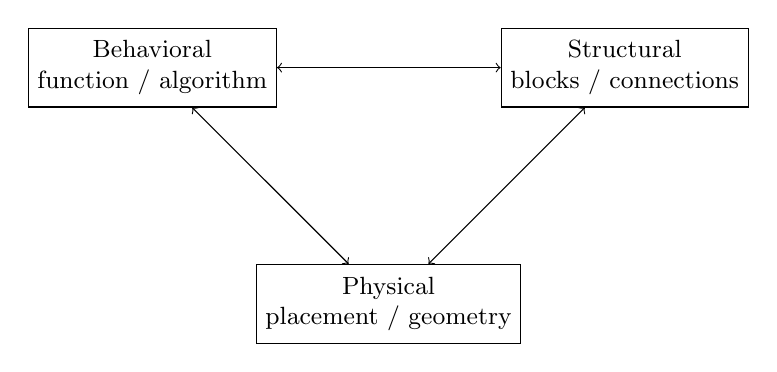
\begin{tikzpicture}[font=\small]
\node[draw,align=center,minimum width=3.1cm,minimum height=1cm] (b) at (-3,1.6) {Behavioral\\function / algorithm};
\node[draw,align=center,minimum width=3.1cm,minimum height=1cm] (s) at (3,1.6) {Structural\\blocks / connections};
\node[draw,align=center,minimum width=3.1cm,minimum height=1cm] (p) at (0,-1.4) {Physical\\placement / geometry};
\draw[<->] (b)--(s);\draw[<->] (b)--(p);\draw[<->] (s)--(p);
\end{tikzpicture}
\end{latin}
\caption{بازنمایی مفهومی رابطه سه دامنه، بر پایه بحث نمودار \lr{Y} کتاب
\cite{weste}. این شکل بازتولید هندسی خود نمودار \lr{Y} نیست؛
تبدیل دامنه‌ها در یک سطح مشخص را برجسته می‌کند.}
\label{fig:design-domains}
\end{figure}

\subsection{مثال بررسی رابط}
فرض کنید بلوکی \lr{MUX} هشت‌بیتی دارد و انتخابش با یک بیت \(S\) انجام می‌شود.
باید معلوم باشد \(S=0\) کدام ورودی را انتخاب می‌کند، هر ورودی چه زمانی معتبر است
و خروجی چه زمانی مصرف می‌شود. اتصال ورودی هفت‌بیتی به آن، یا برداشت معکوس از
معنای \(S\)، می‌تواند عملکرد را عوض کند؛ حتی اگر نام بلوک درست باشد.
در ادامه، همین انضباط را برای رابط پردازنده و حافظه به کار می‌بریم.
